\documentclass[main.tex]{subfiles}
\begin{document}
\section{Analysis}
\lstinputlisting[style=codeStylePy3]{rsa.py}
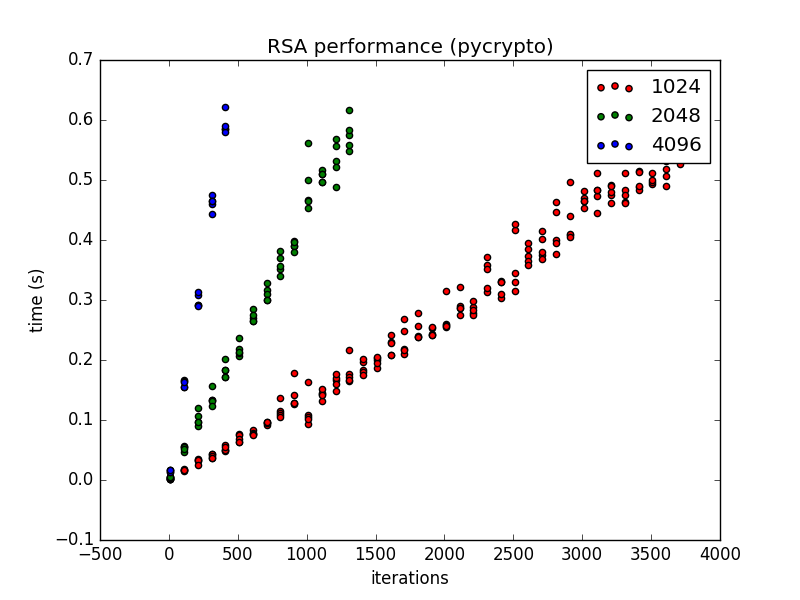
\includegraphics[width=\textwidth]{plot.png}

For all three key sizes, we see that the time taken increases linearly with the
number of iterations. The number of iterations is proportional to the plaintext
size as RSA is a block cipher that encrypts in multiples of $N$ (without
padding the message). If padding were to be used, the time taken would be almost
the same as long as the plaintext size was less than $N$.


\end{document}
